\chapter{General Purpose Input/Outputs}

One of the simplest ways to interface the microcontroller with external circuitry is via General Purpose Input/Outputs (GPIO). The ability for the microcontroller to communicate with external devices via GPIO pins is one of the defining differences between microcontrollers and microprocessors.
Most pins on the microcontroller are able to operate in GPIO mode. As the name implies, a GPIO pin can be either an input or an output. Additionally, a pin can be placed into an alternate function or analogue mode; these will be discussed later.

The microcontroller's GPIO pins are divided up into groups. Each group is known as a port and each port has a letter associated with it (PortA, PortB, etc). Each port contains pins. The maximum number of pins which a port can contain is 16, but some ports contain as few as 2 pins. This means that the name which we assign to a pin is a combination of the port letter and the pin's number in that port. For example: Port A pin 7 refers to a specific pin (shortened to PA7). This naming scheme is useful as the name makes it clear how we interact with that pin. The ports are both a logical and physical division of the pins: all of the pins which belong to a certain port are controlled by a certain block of circuitry which manages that port. The name immediately tells us which block of circuitry our code should interface with in order to control that pin.

A diagram showing how the pin is structured electrically inside the microcontroller is shown in \autoref{fig:gpio}. 
\begin{figure}
\centering
\includegraphics[page=152, clip=true, trim=90 410 90 210, width=\textwidth]{./stm32f0xx_reference_manual}
% left, bottom, right, top
\caption{Internal structure of pin. Source: Figure 17, Reference Manual}
\label{fig:gpio}
\end{figure}

%\begin{overpic}[grid,page=152, trim=90 410 100 210, clip, width=\textwidth]{./stm32f0xx_reference_manual}
%\end{overpic}

\section{Pin Mode}
As mentioned, the pin can be in one of four possible modes: input, output, alternate function, analogue. There is a register which controls which mode the pin operates in, known as the GPIOx\_MODER. The 32 bits of the register are divided up into pairs of bits where each pair of pits sets the mode for the associated pin. 

\subsection{Input Mode}
Input mode is the default mode for most pins. In this mode, the pin is measuring the voltage applied to it and ascertaining whether it is a logic 0 or a logic 1. This "decision" is made by a Schmitt Trigger which has useful characteristics such as well defined high and low levels, hysteresis and high impedance. The logic level of each pin is latched on each clock cycle and written to the Input Data Register (GPIOx\_IDR). As each pin can only be considered to be either a logic high or a logic low, there is only 1 bit necessary to represent the state of a pin.

\subsection{Output Mode}
Here, the pin does not measure a logic level, but rather asserts a logic level. When in output mode, the pin will either assert a logic 0 allowing it to sink current from an external source, or assert a logic 1 allowing it to source current into an external sink. The logic level which is asserted is controlled by the Output Data Register (GPIOx\_ODR). 

Each bit in this register can be set by writing to the register. Additionally, the bits in this register can be set via the Bit Set and Reset Register (GPIOx\_BSSR). This register allows atomic (done in a single instruction) setting or clearing of individual bits in the ODR. 

\subsection{A note on "bricking" your micro}
If you study your dev board circuit diagram carefully, you'll notice that PA13 and PA14 are connected to the debugger. These are the SWD data and SWD clock pins. By default, these pins are not configured as inputs. Rather, they are configured as Alternate Mode, which allows them to be connected to the SWD circuitry inside the STM32F051 and hence serve the purpose of transferring SWD traffic between the SWD peripheral and the ST-Link. If you look at section 9.4.1 of the reference manual, you'll see that in general the reset state of pins is input. Port A is however an exception. Its reset state is 0x2800 0000. This corresponds to all pins as inputs except PA13 and PA14 which are alternate mode. In order for these pins to be connected to the SWD circuitry, they must remain in Alternate Mode. If you set the pins to inputs, they will no longer serve as an interface for the SWD peripheral to the ST-Link. For this reason, you should under no circumstance modify the values of the bits at GPIOA\_MODER[29..36]. 

If you do accidentally set these pins to inputs, it becomes difficult to unset them. As soon as the micro boots up, your code will run and break connectivity with the debugger. The only way to fix this is to intercept the micro before it is able to boot up and erase your bad code from it.
To do this, OpenOCD will be launched with some extra flags to prevent the micro booting up. The OpenOCD command should be executed while the micro is reset to ensure that the pins are back to their default reset state.
\begin{enumerate}
  \item Hold down the reset button. This will force the micro to reset state and prevent your code from running.
  \item Launch OpenOCD with the extra command line arguments: \texttt{-c init -c "reset halt"}
  \item About a quarter of a second after pressing "enter" on that openocd command, release the reset button. OpenOCD should now manage to establish connection.
  \item Connect GDB to OpenOCD. Run the GDB command: \texttt{monitor flash erase\_sector 0 0 last}
  \item Your bad code should now be erased. Power cycle the board, and OpenOCD should be able to connect to it with the normal command.
\end{enumerate}

\section{Pull resistors}
When a pin is set to input mode and there is no logic level applied to it, what value will the bit for that pin in the IDR take on? A logic 1 or a logic 0? Due to the high impedance nature of the pin and the presence of environmental noise, the level which is read from the pin will probably jump randomly between a logic 1 and logic 0. The fact that it's a high impedance input means that even very weak EM signals will cause a voltage to appear on the pin which will cause it to oscillate between logic levels. This is generally bad. In order to define a sort of "default" level which the pin will read when no external signal is applied to it, internal pull-up or pull-down resistors are used. These resistors are selectively turned on or off using the Pull-up/Pull-down Register (GPIOx\_PUPDR).

\subsubsection{How to set or clear individual bits}
\label{sec:set_clear_individual_bits}
There is often a case where you wish to modify only one or two of the bits of a port, leaving the rest of the pins unchanged. If you simply write a pre-defined value to the pins, it will force \emph{all} of them to take on a specific value. The way to modify only a single bit is to do a logic \texttt{AND} or \texttt{OR} of the contents of the register with a pre-defined pattern. An \texttt{OR} has the ability to set specific bits while leaving others unchanged, while and \texttt{AND} has the ability to clear certain bits while leaving the others unchanged. For example, say we wanted to set bits 1 and 2, while clearing bits 0, 3, 4 and 5, leaving the other bits of the port unchanged:
\begin{lstlisting}[fontadjust=true,frame=trBL]
@ assuming Rn contains the address of the register to modify:
LDR R0, [Rn]    
LDR R1, MASK_OUT
ANDS R0, R0, R1
MOVS R1, #0x06
ORRS R0, R0, R1
STR R0, [Rn]
...
.align
MASK_OUT: .word 0b11111111111111111111111111000110
\end{lstlisting}


